\addurlfn{child_process}{\code{child_process}}{https://nodejs.org/api/child_process.html}
\addurlfn{napi}{Node-API}{https://nodejs.org/api/n-api.html}
\addurlfn{node_path}{\code{NODE_PATH}}{https://nodejs.org/api/modules.html}

\addurlfn{rollup}{Rollup.js}{https://rollupjs.org}
\addurlfn{rollup-copy}{\enquote{copy}}{https://npmjs.com/package/rollup-plugin-copy}
\addurlfn{rollup-dts}{\enquote{dts}}{https://npmjs.com/package/rollup-plugin-dts}
\addurlfn{type-declarations}{Typendeklarations-Dateien}{https://typescriptlang.org/docs/handbook/2/type-declarations.html}

\subsubsection{Detaillierte Implementation}

Eine Übersicht der einzelnen Komponenten mit ihren genauen Zusammenhängen wird in Abbildung~\ref{asset:Capacitor-NodeJS:Implementation} dargestellt.

\begin{figure}[H]
    \centering
    \vspace{1em}
    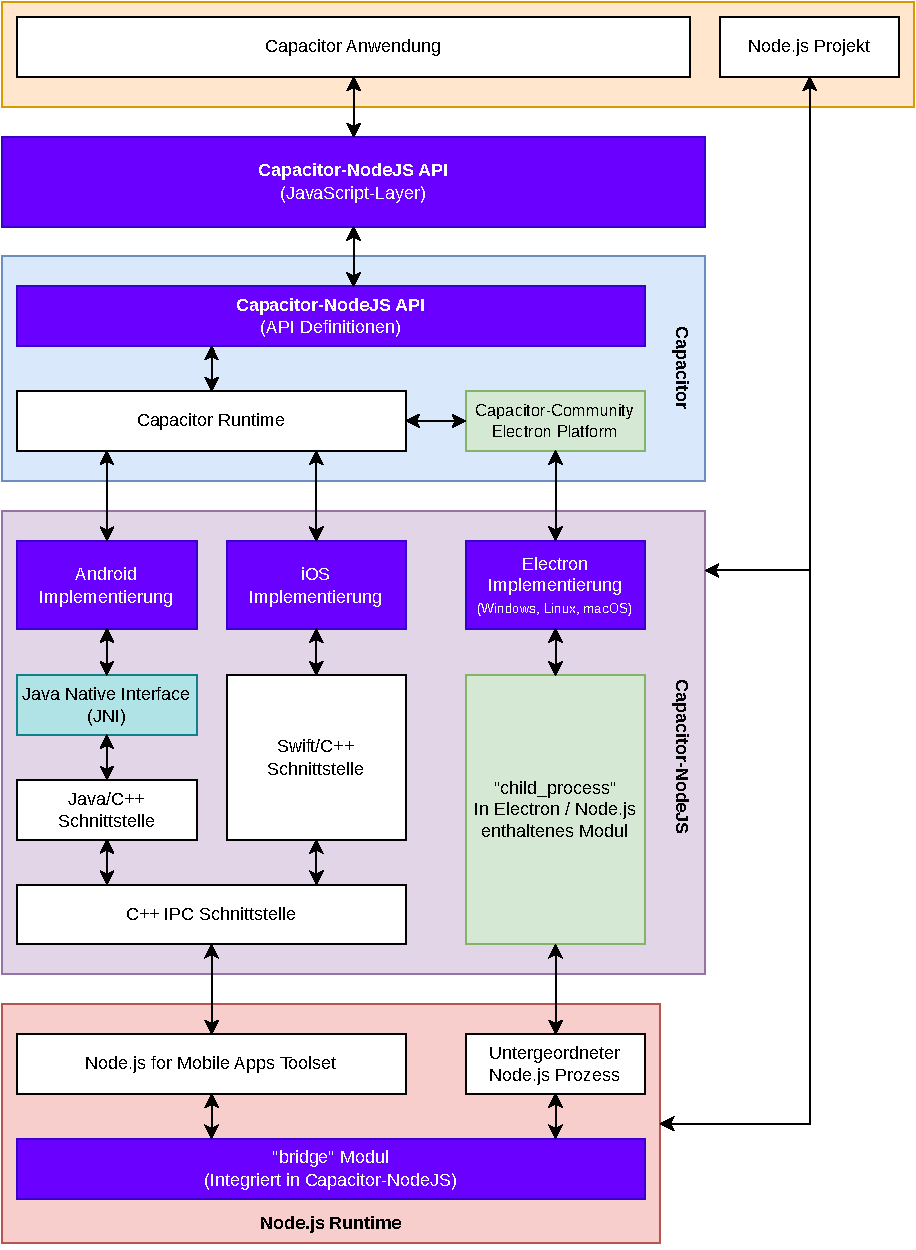
\includegraphics[width=\textwidth]{assets/02_Capacitor-NodeJS/04_Implementation.drawio.pdf}
    \caption[Capacitor-NodeJS / Implementierung]{Implementierung des Capacitor-NodeJS Plugins}
    \label{asset:Capacitor-NodeJS:Implementation}
\end{figure}

\newpage

\paragraph{Plugin API}

Das Capacitor-NodeJS Plugin erweitert seine \ac{api} um einen zusätzlichen JavaScript"=Layer, der zusätzliche nicht-native Funktionen wie das Entfernen bestimmter oder aller Event-Listener implementiert.

\paragraph{Implementierungen}

Um die Implementierung des Plugins auf allen Plattformen übersichtlich und wartungsfreundlich zu gestalten, sind sie in ihrer Struktur sehr ähnlich.
Sie bestehen jeweils aus zwei Teilen:

\begin{enumerate}
    \item Der erste Teil wird von der Capacitor Runtime aufgerufen. Er implementiert die \acs{api}-Struktur und wertet die Parameter der Methoden aus.
    \item Der zweite Teil implementiert die tatsächlichen Funktionen, wie das Starten der Node.js Runtime sowie das Senden und Empfangen von Nachrichten zwischen den Prozessen.
\end{enumerate}

Android Anwendungen sind wie Archive aufgebaut.
Das bedeutet, dass sie aus einer Reihe von Dateien bestehen, die in einem komprimierten Format gespeichert sind.
Daher muss das Node.js Projekt von der Anwendung in das Android Dateisystem kopiert werden, damit die Node.js Runtime darauf zugreifen kann.
\cite{nodejs-mobile:docs}

Um von der Implementierung auf die nativen Binärdateien der Node.js Runtime zuzugreifen, ist unter Android und iOS ein C++ Code als Schnittstelle erforderlich.
Für die Integration nativen Codes unter Android ist zusätzlich das \ac{ndk} erforderlich.
Der verwendete Code für die Schnittstelle stammt aus der Dokumentation des Node.js for Mobile Apps Toolsets.
\cite{nodejs-mobile:docs}

In der Electron Implementierung wird das in Electron bzw.\ Node.js enthaltene Modul \fn{child_process} verwendet, um einen Node.js Unterprozess zu starten.

\begin{note}
    Die offizielle Entwicklungsumgebung für iOS, Xcode, ist ausschließlich für macOS verfügbar.~\cite{xcode:support}
    Da während der Entwicklung nur Windows- und Linux-Geräte zur Verfügung standen, war das Implementieren und Testen des Plugins für iOS nicht möglich.
\end{note}

\newpage

\paragraph{Interprozesskommunikation}

Die Kommunikation zwischen dem Node.js Projekt und der Capacitor Anwendung erfordert unter Android und iOS erneut nativen C++ Code.
Dieser Code dient als \ac{ipc} Schnittstelle und ist von der Plugin"=Implementierung aufrufbar und über die \fn{napi} auch für JavaScript-Code in der Node.js Runtime zugänglich.
Dadurch kann eine Art Event-Emitter realisiert werden.

Der verwendete Code für die \ac{ipc} Schnittstelle stammt aus dem Node.js for Mobile Apps Cordova Plugin.
\cite{nodejs-mobile-cordova}

\vspace{1em}

\begin{figure}[H]
    \centering
    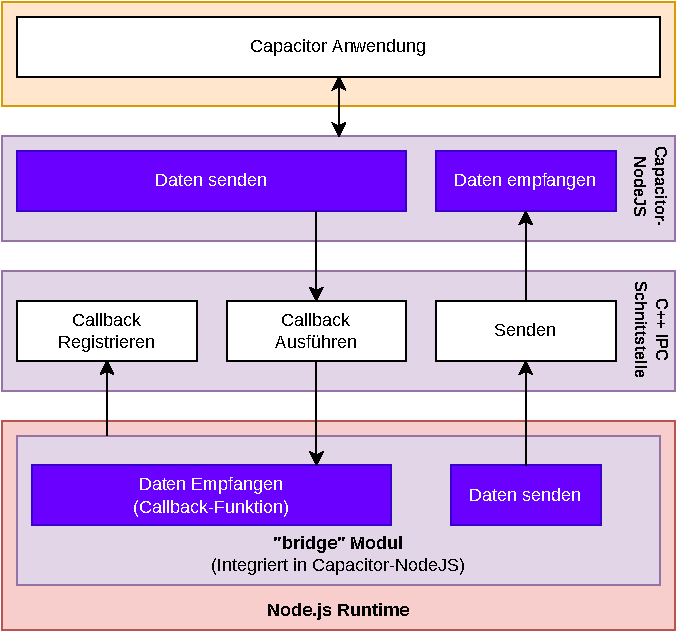
\includegraphics[width=0.85\textwidth]{assets/02_Capacitor-NodeJS/03_Interprozesskommunikation.drawio.pdf}
    \caption[Capacitor-NodeJS / Interprozesskommunikation]{Interprozesskommunikation zwischen der Capacitor Anwendung, dem Capacitor-NodeJS Plugin und der Node.js Runtime.}
\end{figure}

Um Daten von der Capacitor Anwendung zu empfangen, registriert ein JavaScript-Code in der nativen \ac{ipc} Schnittstelle eine Callback-Funktion.
Das Capacitor-NodeJS Plugin kann dann eine Funktion von der Schnittstelle mit Nutzdaten aufrufen.
Diese Funktion leitet die Daten an die JavaScript"=Callback"=Funktion weiter.

Um Daten an die Capacitor Anwendung zu senden, ruft der JavaScript-Code in der Schnittstelle eine Funktion mit Nutzdaten auf.
Diese Funktion leitet die Daten an das Capacitor-NodeJS Plugin weiter.

In der Electron"=Implementierung wird die Kommunikation zum untergeordneten Node.js Prozess durch das \fn{child_process} Modul verwaltet.

Um die Benutzerfreundlichkeit zu verbessern, wurde der JavaScript-Code für die Handhabung der Kommunikation sowie für die Serialisierung und Deserialisierung der Nutzdaten mittels \ac{json} in das \code{bridge} Modul verlagert.
Es erweitert die Node.js Event-Emitter Klasse, um die Kompatibilität mit vorhandenen Projekten zu verbessern.
Das Modul wird automatisch geladen, so dass Benutzer keine zusätzlichen Schritte ausführen müssen.

Das \code{bridge} Modul wird mit \fn{rollup} gebündelt und mit dem Rollup plugin \fn{rollup-copy} in die Unterverzeichnisse der jeweiligen Plattformen kopiert.
Um auch eine TypeScript Unterstützung zu gewährleisten, wird mit dem Rollup plugin \fn{rollup-dts} ein zusätzliches Paket erstellt, das nur die \fn{type-declarations} enthält, um Informationen über die \ac{api} zu liefern.

Um das automatische Laden von Modulen zu ermöglichen, wird beim Start der Runtime die Umgebungsvariable \fn{node_path} gesetzt.
Diese Umgebungsvariable enthält eine Liste von Pfaden, die durch ein Semikolon getrennt sind.
Node.js durchsucht diese Pfade nach Modulen, die im Node.js Projekt nicht gefunden wurden.
\cite{nodejs-mobile:docs, nodejs}

\printfn
